\documentclass{beamer}
%\usepackage{beamerarticle}

\usepackage[ngerman]{babel}
\usepackage[utf8]{inputenc}
\usepackage[T1]{fontenc}
\usepackage{tikz}
\usetikzlibrary{positioning, arrows}
\usepackage{listings}
\usepackage{fancybox}
\usepackage{verbatim}

\usepackage{pifont}% http://ctan.org/pkg/pifont
\newcommand{\cmark}{\ding{51}}%
\newcommand{\xmark}{\ding{55}}%

\usetheme{Madrid}
\setbeamercovered{transparent}

\title[SWT-Praktikum]{Pr\"sentationen mit dem Paktet  Beamer}
\author{swp15.gkp}
\date{\today{}}
%\logo{\includegraphics[scale=0.25]{logo}}

\begin{document}
\begin{frame}
\center \huge \textbf{Kartenbasiertes Multiplayerspiel} \\
\end{frame}

\begin{frame}{Überblick}
\begin{itemize}
\item Retrospektive
\item Perpektive
\begin{itemize}
\item Phaser
\item Struktur- und Entwurfsprinzipien
\item Überbick Implementierungsphase
\item Qualitätssicherung
\end{itemize}
\end{itemize}
\end{frame}

\begin{frame}{Produktübersicht -Retrospektiv}
\begin{figure}[htb]
  \centering
  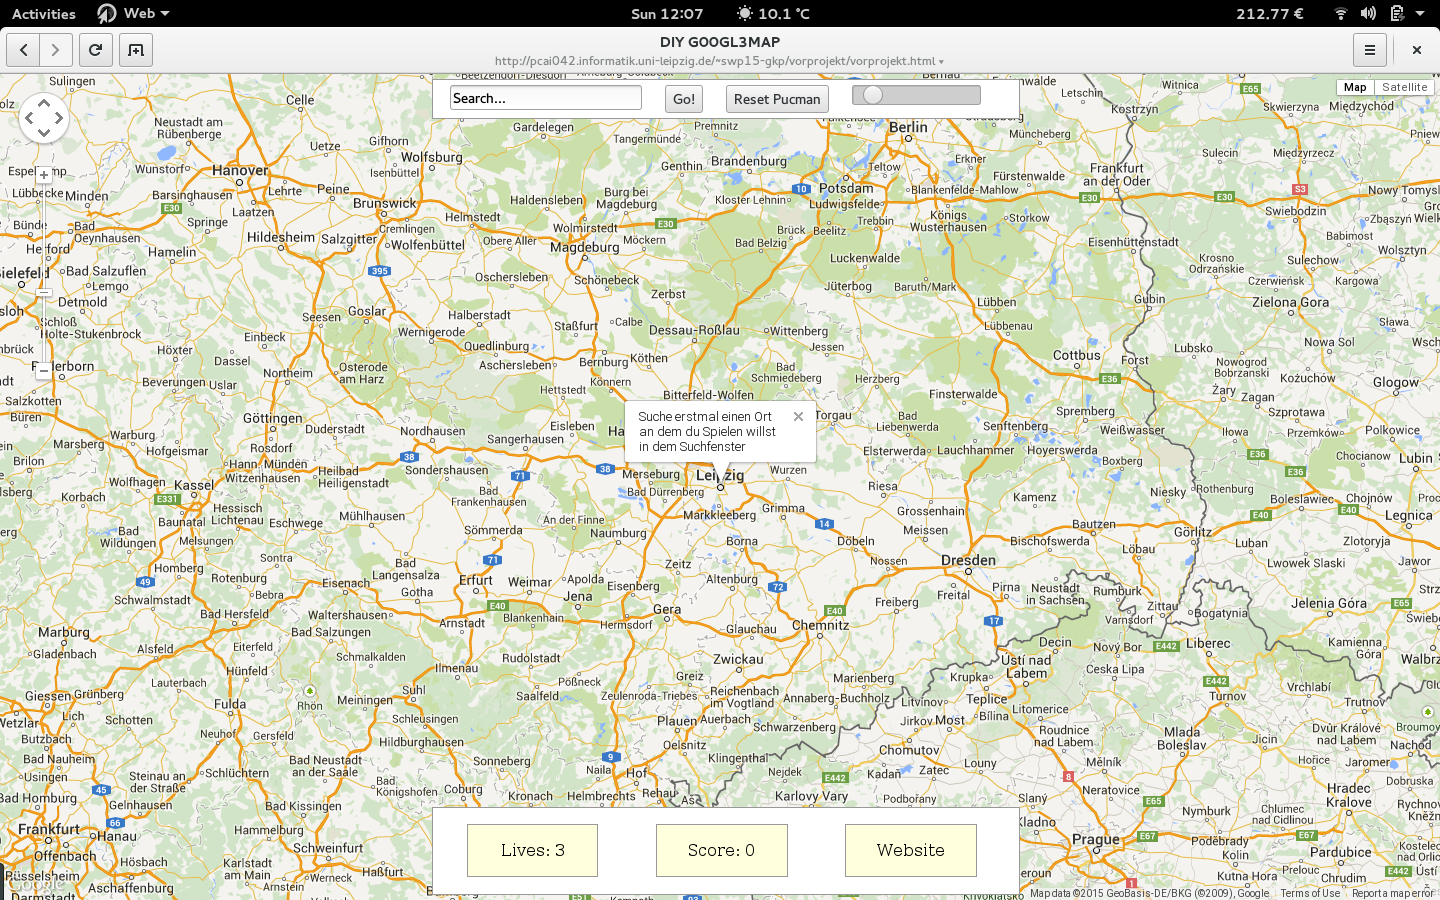
\includegraphics[scale=0.18]{1.png}
%\caption{der rote Punkt bezeichnet unser gesuchtes Teilwort}
  \label{PNFs}
\end{figure} 
\begin{itemize}
\item Zugriff über Spiele-Website auf das Programm
\item Suchfeld
\item  Reset und Lautstärke
\item Anzeige der Highscore und der verbleibenden Leben  
\end{itemize}
\end{frame}
\begin{frame}{Persepektive}
\begin{figure}[htb]
  \centering
  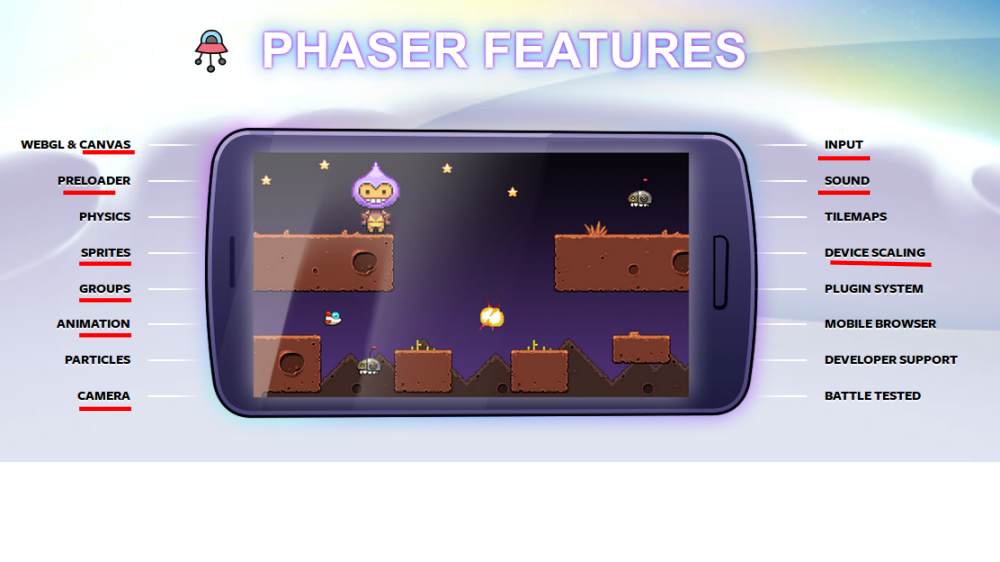
\includegraphics[scale=0.48]{3.png}
%\caption{der rote Punkt bezeichnet unser gesuchtes Teilwort}
  \label{PNFs}
\end{figure} 
\end{frame}
\begin{frame}{Persepektive}
\begin{figure}[htb]
  \centering
  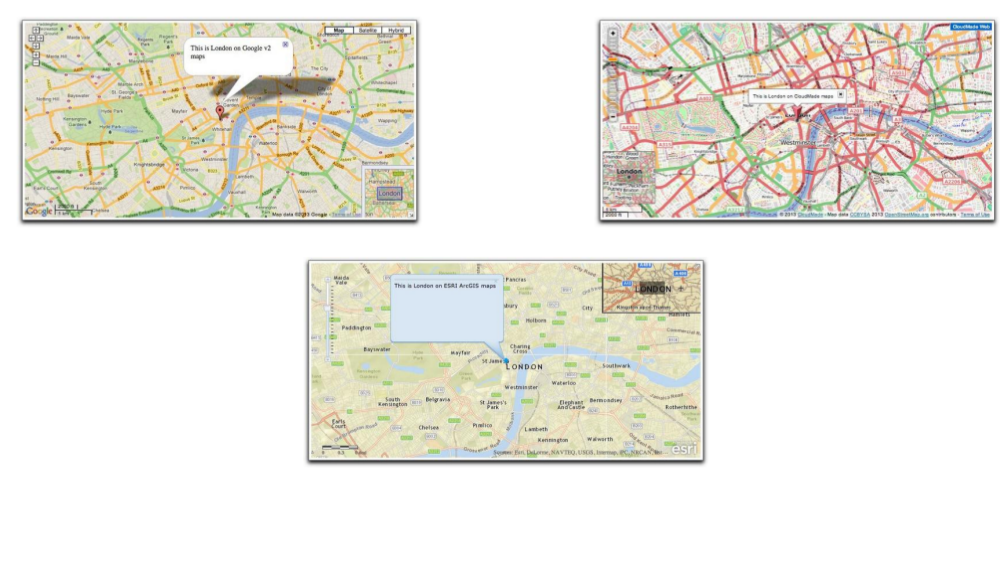
\includegraphics[scale=0.48]{4.png}
%\caption{der rote Punkt bezeichnet unser gesuchtes Teilwort}
  \label{PNFs}
\end{figure} 
\end{frame}
\begin{frame}{Persepektive}
\begin{figure}[htb]
  \centering
  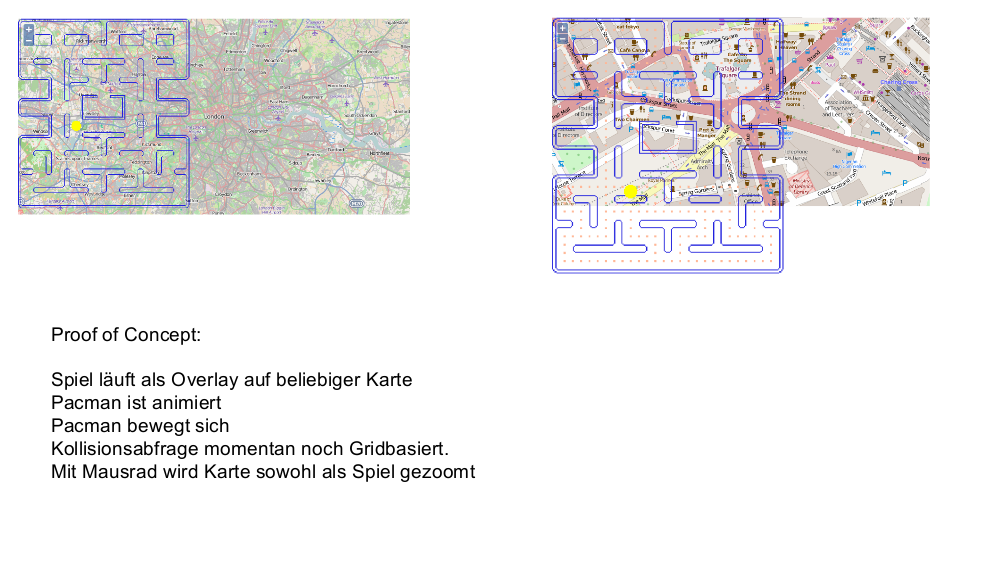
\includegraphics[scale=0.48]{5.png}
%\caption{der rote Punkt bezeichnet unser gesuchtes Teilwort}
  \label{PNFs}
\end{figure} 
\end{frame}

\begin{frame}{Persepektive - Struktur- und
Entwurfsprinzipien}
\begin{figure}[htb]
  \centering
  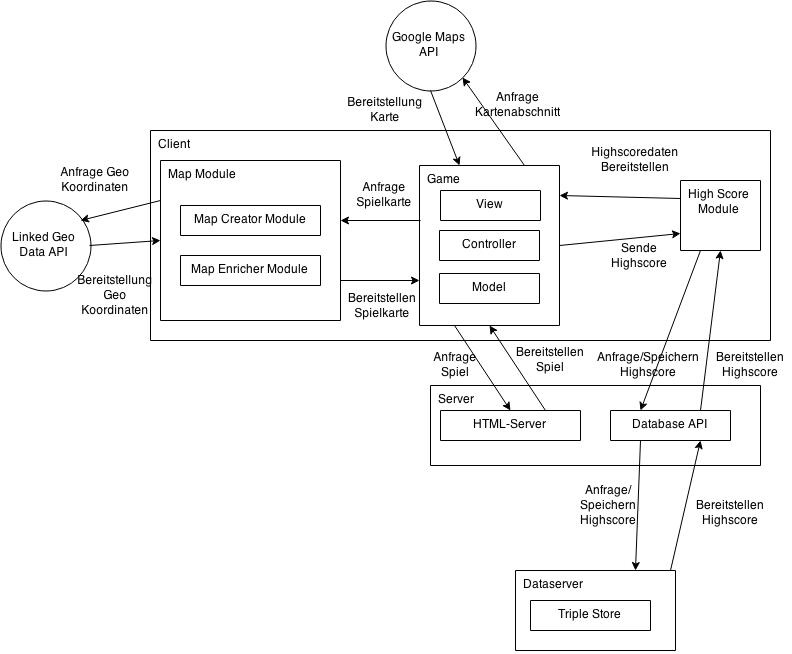
\includegraphics[scale=0.34]{6.png}
%\caption{der rote Punkt bezeichnet unser gesuchtes Teilwort}
  \label{PNFs}
\end{figure} 
\end{frame}
\begin{frame}{Server}
\begin{itemize}
\item Spieldateien
\item  Verarbeitung von Highscoreanfragen 
\item Database API - Weiterleitung von Manipulationen zwischen dem Dataserver und dem Client  
\end{itemize}
\end{frame}
\begin{frame}{Client - Gameblock}
angelehnt an das MVC Prinzip, nutzt Phaser \par\bigskip

\begin{itemize}
\item model
\begin{itemize}
\item Enthält die darzustellenden Daten.
\item Unabhängig von den anderen Schichten.
\end{itemize}
\item view
\begin{itemize}
\item Darstellung der benötigten
Daten aus dem Modell.
\item Entgegennahme von Benutzerinteraktionen 
\end{itemize}

\item controller
\begin{itemize}
\item Verwaltet die Präsentation
\item und Benutzeraktionen.
\end{itemize}

\end{itemize}
\end{frame}

\begin{frame}{Client - weitere Module}
\begin{itemize}
\item Highscore Modul
\begin{itemize}
\item Verwaltet die Highscores der Spieler.
\item Anfragen an den Server zum Triplestore.
\item 
\end{itemize}
\item Linked GeoData API
\begin{itemize}
\item Extrahiert aus OpenStreetMap die Geo-Daten für
das Erstellen des Spiel-Levels.
\end{itemize}
\item Map Module
\begin{itemize}
\item Map Creator Modul
\begin{itemize}
\item Bildet den Graphen des Levels aus den Straßenzügen.
\end{itemize}

\item Map Enricher Modul
\begin{itemize}
\item Bindet semantische Daten
in die Kartenerstellung ein.
\end{itemize}
\item Geo-Daten die von der GeoData API.
\end{itemize}
\end{itemize}

\end{frame}

\begin{frame}{Google Maps API}
Übernimmt das Anzeigen
der Karte sowie das Suchen des eingegebenen Ortes. \par\bigskip

Die integrierten Steuerelemente sind bei der Suche nach einem geeigneten
Spielort verfügbar, danach werden die Elemente deaktiviert um einen
füssigen Spielbetrieb zu gewährleisten.

\end{frame}

\begin{frame}{kurzer Überblick über die Implementierungsphase}
\begin{itemize}
\item ab Woche 1
\begin{itemize}
\item Leveldarstellung
\item Vorprojekt in Phaser
\end{itemize}
\item ab Woche 2
\begin{itemize}
\item Mapmodul
\end{itemize}
\item ab Woche 3
\begin{itemize}
\item Semantische Daten
\end{itemize}
\item ab Woche 4
\begin{itemize}
\item Geister
\item Powerups
\end{itemize}
\item ab Woche 5
\begin{itemize}
\item Alles war auf der Strecke blieb.
\item Debuggen
\end{itemize}
\end{itemize}
\end{frame}

\begin{frame}{Qualitätssicherung - Anforderungen}
\begin{center}
    \begin{tabular}{ | l | c | c | c | c | c | c | c | }
    \hline
     Produktqualität & Relevant & Nicht relevant \\ \hline
	 Funktionalität   & \cmark & \\ \hline
	 Zuverlässigkeit  &  & \cmark  \\ \hline	
	 Benutzbarkeit & \cmark &  \\ \hline
	 Effizienz & & \cmark  \\ \hline
	 Änderbarkeit &  \cmark &  \\ \hline
	 Übertragbarkeit &  \cmark & \\ \hline
	 
    \end{tabular}
\end{center}

\end{frame}
\begin{frame}{Qualitätssicherung - Codingstandards}
\begin{itemize}
\item Code in Java Script
\item -> Code Conventions für Java Script
\item \url{http://javascript.crockford.com/code.html}
\item inspiriert durch die Sun document Code Conventions für Java
\item beinhaltet auch Quelltextdokumentation

\end{itemize}
\end{frame}

\begin{frame}{Beispielcode}
\begin{figure}[htb]
  \centering
  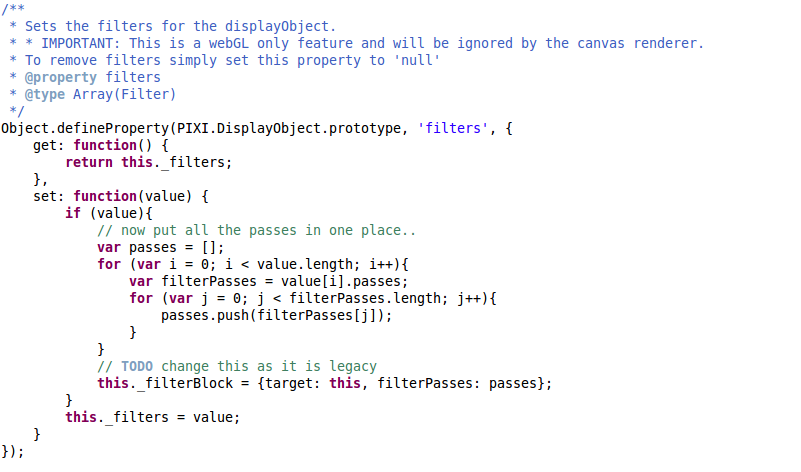
\includegraphics[scale=0.4]{7.png}
%\caption{der rote Punkt bezeichnet unser gesuchtes Teilwort}
  \label{PNFs}
\end{figure} 

\end{frame}
\begin{frame}
\Huge \center \textbf{F R A G E N ?}
\end{frame}
\end{document}